\documentclass[a4paper,article, oneside]{memoir}
\usepackage[danish]{babel} % load typographical rules for the english language
\usepackage{graphics} % for \scalebox
\usepackage{hyperref} % for \href
\usepackage{xcolor} % for text color
\usepackage{enumitem} % for ordered and unordered list
\usepackage{graphicx} % for images
\usepackage{pdfpages} % for including pdfs
\usepackage{footnote} % for footnotes
\usepackage{longtable} % for tabular environment that spans multiple pages and supports footnotes
\usepackage{colortbl} % for cell coloring
\usepackage{multirow} % for \multicolumn

% https://github.com/latex3/babel/issues/51
\makeatletter\AtBeginDocument{\let\@elt\relax}\makeatother

% styling
\setsecnumdepth{subsubsection} % how deep to number sections
\setlength{\parindent}{0em} % horizontal indent for first line of paragraph
\setlength{\parskip}{1em} % vertical space between paragraphs

\newcommand{\textdesc}[1]{\textit{\textbf{#1}}}
\newcommand{\descitem}[1]{\item \textdesc{#1}}

\title{\documenttitle\\\scalebox{0.85}{\documentsubtitle}}
\author{Aslak Johansen \href{mailto:asjo@mmmi.sdu.dk}{asjo@mmmi.sdu.dk}\\Aisha Umair \href{mailto:aiu@mmmi.sdu.dk}{aiu@mmmi.sdu.dk}}

\begin{document}

\maketitle
\setcounter{tocdepth}{2}
\tableofcontentswrapper

\section*{Formål og Mål}

Formålet med problemanalysefasen er at få udarbejdet gruppens projektgrundlag. Når I er færdige med fasen, så har projektgruppen


\begin{itemize}
  \item gennemført problemanalyse
  \item foretaget metodevalg
  \item planlagt projektet overordnet
    \end{itemize}
 og projektgruppen har på grundlag heraf lavet og fået godkendt

    \begin{itemize}
      \item projektgrundlaget
\end{itemize}

\section*{Opgaver i fasen}

\textbf{Problemanalyse}\\
Problemanalysen handler  om at forstå projektets udgangspunkt og at finde det problem, der passer til projektet og som projektgruppen har en fælles interesse i at arbejde med. Problemanalysen handler også om at undersøge den løsningsramme, World of Zuul, som er er sat op for projektet.
\\
\\ Benyt e-tivitet 03 Problemorienteret projektarbejde, 04 Problemanalyse og problemformulering, 05 Projektets faglige vidensgrundlag  fra ProOnline til at forstå hvad problemorienteret projektarbejde er og til at lave problemanalyse. 

\textbf{Metodevalg og overordnet projektplan}\\
Metodevalget er afgørende for projektforløbet, fordi metoden er svaret på, hvordan I vil løse projektets problem. Den overordnede projektplan laves som en tids- og aktivitetsplan for hovedaktiviteterne  i projektarbejdet. 
\\
\\ Benyt e-tivitet 06 Metoder og planlægning i projektarbejdet til at gennemføre metodevalg og til at lave en overordnet plan for projektet.

\textbf{Projektgrundlag}\\
Projektgrundlaget udarbejdes dels som foreløbige kapitler i den endelige projektrapport. dels som en poster. Det er kun posteren, der afleveres i denne fase. 
\\ De foreløbig kapitler, som skal udarbejdes, er: 
 \begin{itemize}
      \item Forside med titel
      \item Introduktion
      \item Problemformulering
      \item Afgrænsninger
      \item Begrebsdefinitioner, teori og faglig litteratur
      \item Projektets metode
\end{itemize}
Læs nærmere om projektrapporten og de relevante afsnit i \url{https://ibog3.gyldendal.dk/projekterograpporter#/double/212/}
\\ Posteren præsenterer hovedpunkter fra projektgrundlaget.  Posteren udarbejdes vha. følgende skabelon Projektgrundlag \hyperref[sec:p]{(poster)}. Posteren udarbejdes i A0 format og og printes vha. A0 printer. Se opsætning her \ref{fig:poster}
\begin{figure}[htb]
\begin{center}
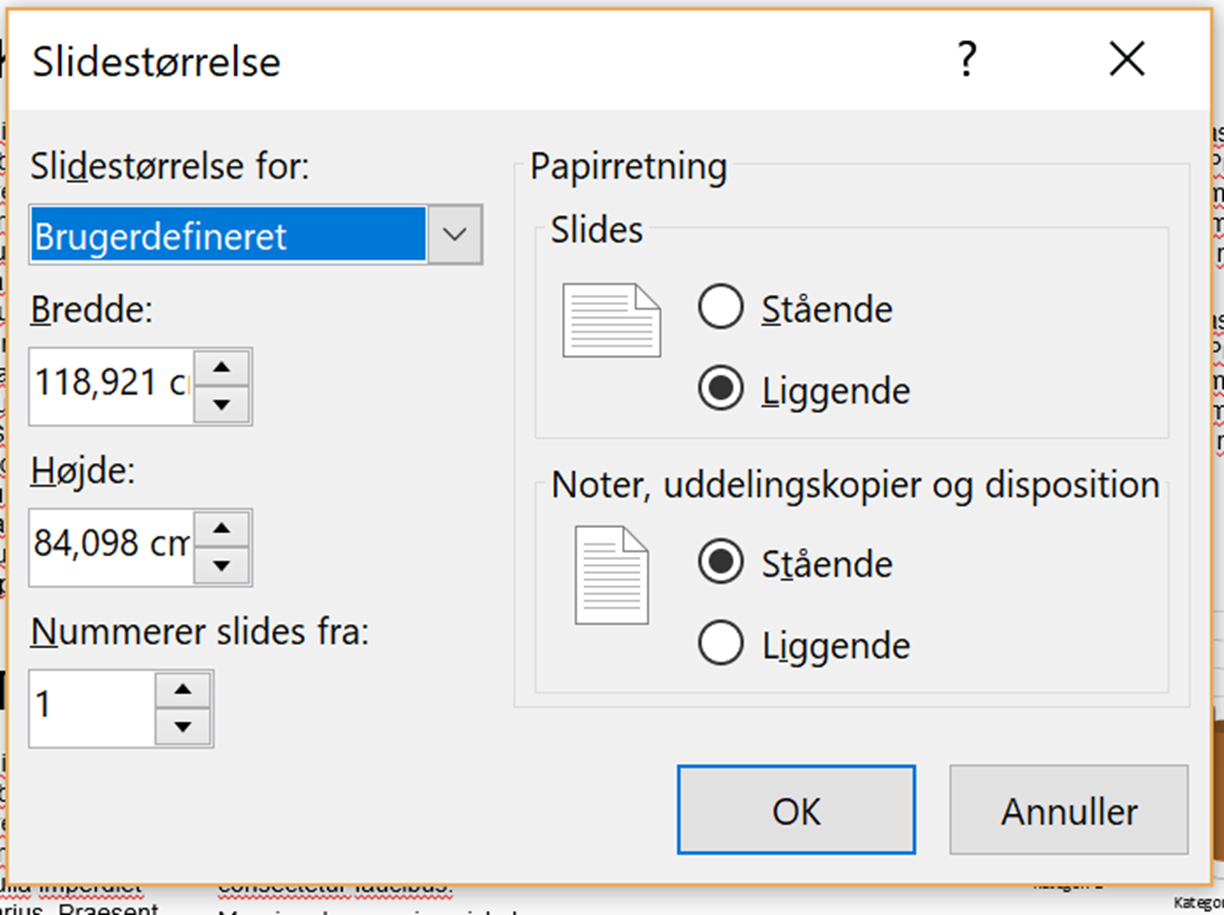
\includegraphics[width=10cm]{images/postersize.png}
\caption{Slidestørrelse}\label{fig:poster}
\end{center}
\end{figure}

 Der står fx en A0 printer i printerrummet ved siden af personalefrokostrummet. Se vejledningen i rummet. Posteren præsenteres på et projektseminar. Posteren opdateres og afleveres efter projektseminaret. Vi anbefaler, at I udskriver den opdaterede poster og hænger den op ved jeres projektarbejdsplads.

\section*{Aktiviteter i fasen}

\documentclass[a4paper,article, oneside]{memoir}
\usepackage[danish]{babel} % load typographical rules for the english language
\usepackage{graphics} % for \scalebox
\usepackage{hyperref} % for \href
\usepackage{xcolor} % for text color
\usepackage{enumitem} % for ordered and unordered list
\usepackage{graphicx} % for images
\usepackage{pdfpages} % for including pdfs
\usepackage{footnote} % for footnotes
\usepackage{longtable} % for tabular environment that spans multiple pages and supports footnotes
\usepackage{colortbl} % for cell coloring
\usepackage{multirow} % for \multicolumn

% https://github.com/latex3/babel/issues/51
\makeatletter\AtBeginDocument{\let\@elt\relax}\makeatother

% styling
\setsecnumdepth{subsubsection} % how deep to number sections
\setlength{\parindent}{0em} % horizontal indent for first line of paragraph
\setlength{\parskip}{1em} % vertical space between paragraphs

\newcommand{\textdesc}[1]{\textit{\textbf{#1}}}
\newcommand{\descitem}[1]{\item \textdesc{#1}}

\title{\documenttitle\\\scalebox{0.85}{\documentsubtitle}}
\author{Aslak Johansen \href{mailto:asjo@mmmi.sdu.dk}{asjo@mmmi.sdu.dk}\\Aisha Umair \href{mailto:aiu@mmmi.sdu.dk}{aiu@mmmi.sdu.dk}}

\begin{document}

\maketitle
\setcounter{tocdepth}{2}
\tableofcontentswrapper


\section*{Formål og Mål}

Formålet med problemanalysefasen er at få udarbejdet gruppens projektgrundlag. Når I er færdige med fasen, så har projektgruppen

\begin{itemize}
  \item gennemført en problemanalyse
  \item foretaget et metodevalg
  \item planlagt projektet overordnet
\end{itemize}

og projektgruppen har på grundlag heraf lavet og fået godkendt projektgrundlaget.

\section*{Opgaver i Fasen}

\subsection*{Problemanalyse}

Problemanalysen handler  om at forstå projektets udgangspunkt og at finde den problemstilling, der både passer til projektet og som projektgruppen har en fælles interesse i at arbejde med. Problemanalysen handler også om at undersøge den løsningsramme, World of Zuul, som er er sat op for projektet.

Benyt modulerne \say{03 Problemorienteret projektarbejde}, \say{04 Problemanalyse og problemformulering}, og \say{05 Projektets faglige vidensgrundlag} fra ProOnline til at forstå hvad problemorienteret projektarbejde er og til at lave problemanalysen.

\subsection*{Metodevalg og Overordnet Projektplan}

Metodevalget er afgørende for projektforløbet, fordi metoden er svaret på, hvordan I vil løse projektets problem. Den overordnede projektplan laves som en tids- og aktivitetsplan for hovedaktiviteterne i projektarbejdet.

Benyt moduler \say{06 Metoder og planlægning i projektarbejdet} fra ProOnline til at gennemføre metodevalg og til at lave en overordnet plan for projektet.

\subsection*{Projektgrundlag}

Projektgrundlaget udarbejdes dels som foreløbige kapitler i den endelige projektrapport, og dels som en \textsl{poster}. Det er kun posteren, der afleveres i denne fase.

De foreløbig kapitler, som skal udarbejdes, er:
\begin{itemize}
  \item Forside med titel
  \item Introduktion
  \item Problemformulering
  \item Afgrænsninger
  \item Begrebsdefinitioner, teori og faglig litteratur
  \item Projektets metode
\end{itemize}

Læs nærmere om projektrapporten og de relevante afsnit i følgende link:\\
\url{https://projekterograpporterpaatekniskeudd-2udg.digi.hansreitzel.dk/?id=156}

Posteren præsenterer hovedpunkter fra projektgrundlaget.
%Posteren udarbejdes vha. følgende skabelon Projektgrundlag \hyperref[sec:p]{(poster)}.
Posteren udarbejdes i A0 format og printes. %Se opsætning her i figur \ref{fig:poster}.

%\begin{figure}[htb]
%  \begin{center}
%    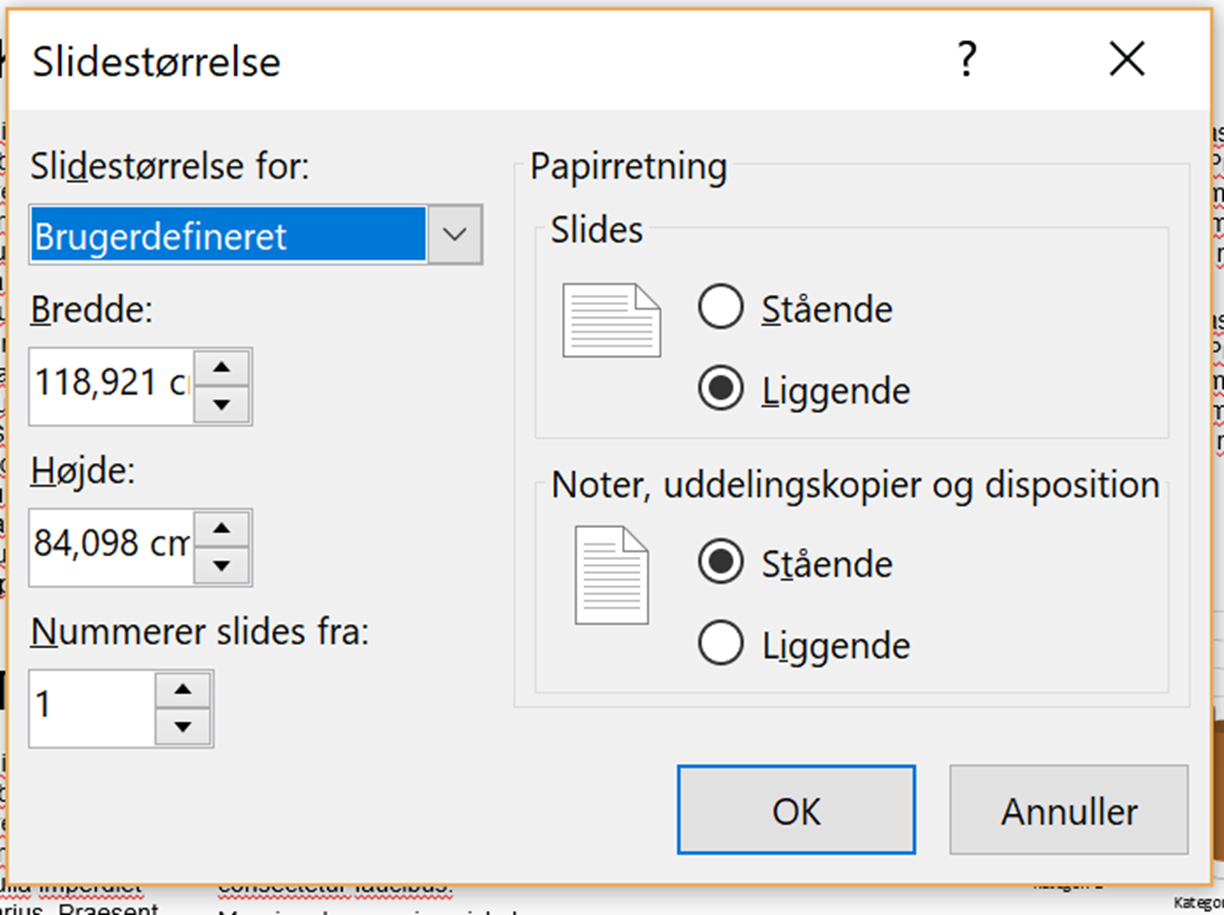
\includegraphics[width=10cm]{images/postersize.png}
%    \caption{Slidestørrelse}\label{fig:poster}
%  \end{center}
%\end{figure}

%Der står fx en A0 printer i printerrummet ved siden af personalefrokostrummet. Se vejledningen i rummet. Posteren præsenteres på et projektseminar. Posteren opdateres og afleveres efter projektseminaret. Vi anbefaler, at I udskriver den opdaterede poster og hænger den op ved jeres projektarbejdsplads.

\section*{Aktiviteter i fasen}

\documentclass[a4paper,article, oneside]{memoir}
\usepackage[danish]{babel} % load typographical rules for the english language
\usepackage{graphics} % for \scalebox
\usepackage{hyperref} % for \href
\usepackage{xcolor} % for text color
\usepackage{enumitem} % for ordered and unordered list
\usepackage{graphicx} % for images
\usepackage{pdfpages} % for including pdfs
\usepackage{footnote} % for footnotes
\usepackage{longtable} % for tabular environment that spans multiple pages and supports footnotes
\usepackage{colortbl} % for cell coloring
\usepackage{multirow} % for \multicolumn

% https://github.com/latex3/babel/issues/51
\makeatletter\AtBeginDocument{\let\@elt\relax}\makeatother

% styling
\setsecnumdepth{subsubsection} % how deep to number sections
\setlength{\parindent}{0em} % horizontal indent for first line of paragraph
\setlength{\parskip}{1em} % vertical space between paragraphs

\newcommand{\textdesc}[1]{\textit{\textbf{#1}}}
\newcommand{\descitem}[1]{\item \textdesc{#1}}

\title{\documenttitle\\\scalebox{0.85}{\documentsubtitle}}
\author{Aslak Johansen \href{mailto:asjo@mmmi.sdu.dk}{asjo@mmmi.sdu.dk}\\Aisha Umair \href{mailto:aiu@mmmi.sdu.dk}{aiu@mmmi.sdu.dk}}

\begin{document}

\maketitle
\setcounter{tocdepth}{2}
\tableofcontentswrapper


\section*{Formål og Mål}

Formålet med problemanalysefasen er at få udarbejdet gruppens projektgrundlag. Når I er færdige med fasen, så har projektgruppen

\begin{itemize}
  \item gennemført en problemanalyse
  \item foretaget et metodevalg
  \item planlagt projektet overordnet
\end{itemize}

og projektgruppen har på grundlag heraf lavet og fået godkendt projektgrundlaget.

\section*{Opgaver i Fasen}

\subsection*{Problemanalyse}

Problemanalysen handler  om at forstå projektets udgangspunkt og at finde den problemstilling, der både passer til projektet og som projektgruppen har en fælles interesse i at arbejde med. Problemanalysen handler også om at undersøge den løsningsramme, World of Zuul, som er er sat op for projektet.

Benyt modulerne \say{03 Problemorienteret projektarbejde}, \say{04 Problemanalyse og problemformulering}, og \say{05 Projektets faglige vidensgrundlag} fra ProOnline til at forstå hvad problemorienteret projektarbejde er og til at lave problemanalysen.

\subsection*{Metodevalg og Overordnet Projektplan}

Metodevalget er afgørende for projektforløbet, fordi metoden er svaret på, hvordan I vil løse projektets problem. Den overordnede projektplan laves som en tids- og aktivitetsplan for hovedaktiviteterne i projektarbejdet.

Benyt moduler \say{06 Metoder og planlægning i projektarbejdet} fra ProOnline til at gennemføre metodevalg og til at lave en overordnet plan for projektet.

\subsection*{Projektgrundlag}

Projektgrundlaget udarbejdes dels som foreløbige kapitler i den endelige projektrapport, og dels som en \textsl{poster}. Det er kun posteren, der afleveres i denne fase.

De foreløbig kapitler, som skal udarbejdes, er:
\begin{itemize}
  \item Forside med titel
  \item Introduktion
  \item Problemformulering
  \item Afgrænsninger
  \item Begrebsdefinitioner, teori og faglig litteratur
  \item Projektets metode
\end{itemize}

Læs nærmere om projektrapporten og de relevante afsnit i følgende link:\\
\url{https://projekterograpporterpaatekniskeudd-2udg.digi.hansreitzel.dk/?id=156}

Posteren præsenterer hovedpunkter fra projektgrundlaget.
%Posteren udarbejdes vha. følgende skabelon Projektgrundlag \hyperref[sec:p]{(poster)}.
Posteren udarbejdes i A0 format og printes. %Se opsætning her i figur \ref{fig:poster}.

%\begin{figure}[htb]
%  \begin{center}
%    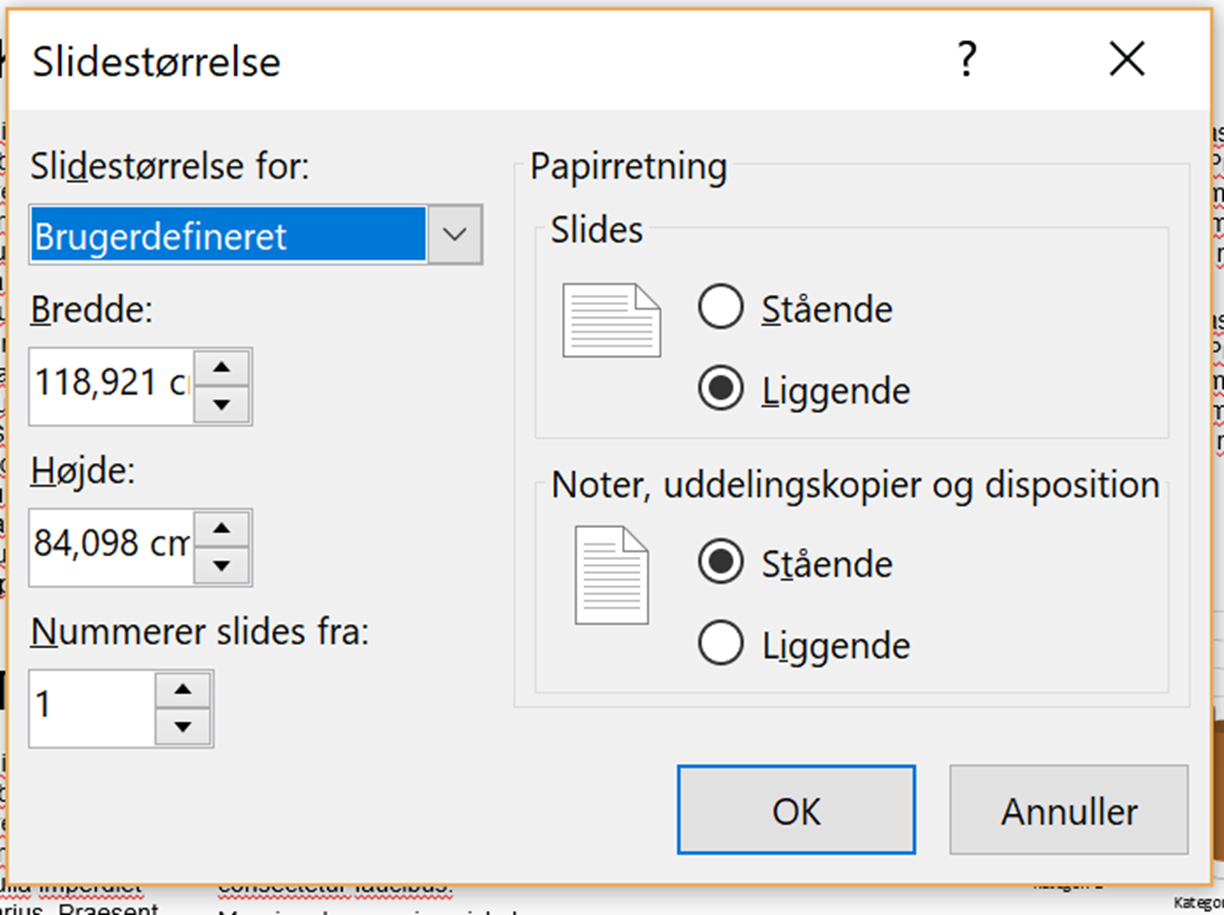
\includegraphics[width=10cm]{images/postersize.png}
%    \caption{Slidestørrelse}\label{fig:poster}
%  \end{center}
%\end{figure}

%Der står fx en A0 printer i printerrummet ved siden af personalefrokostrummet. Se vejledningen i rummet. Posteren præsenteres på et projektseminar. Posteren opdateres og afleveres efter projektseminaret. Vi anbefaler, at I udskriver den opdaterede poster og hænger den op ved jeres projektarbejdsplads.

\section*{Aktiviteter i fasen}

\documentclass[a4paper,article, oneside]{memoir}
\include{shared}

\section*{Formål og Mål}

Formålet med problemanalysefasen er at få udarbejdet gruppens projektgrundlag. Når I er færdige med fasen, så har projektgruppen

\begin{itemize}
  \item gennemført en problemanalyse
  \item foretaget et metodevalg
  \item planlagt projektet overordnet
\end{itemize}

og projektgruppen har på grundlag heraf lavet og fået godkendt projektgrundlaget.

\section*{Opgaver i Fasen}

\subsection*{Problemanalyse}

Problemanalysen handler  om at forstå projektets udgangspunkt og at finde den problemstilling, der både passer til projektet og som projektgruppen har en fælles interesse i at arbejde med. Problemanalysen handler også om at undersøge den løsningsramme, World of Zuul, som er er sat op for projektet.

Benyt modulerne \say{03 Problemorienteret projektarbejde}, \say{04 Problemanalyse og problemformulering}, og \say{05 Projektets faglige vidensgrundlag} fra ProOnline til at forstå hvad problemorienteret projektarbejde er og til at lave problemanalysen.

\subsection*{Metodevalg og Overordnet Projektplan}

Metodevalget er afgørende for projektforløbet, fordi metoden er svaret på, hvordan I vil løse projektets problem. Den overordnede projektplan laves som en tids- og aktivitetsplan for hovedaktiviteterne i projektarbejdet.

Benyt moduler \say{06 Metoder og planlægning i projektarbejdet} fra ProOnline til at gennemføre metodevalg og til at lave en overordnet plan for projektet.

\subsection*{Projektgrundlag}

Projektgrundlaget udarbejdes dels som foreløbige kapitler i den endelige projektrapport, og dels som en \textsl{poster}. Det er kun posteren, der afleveres i denne fase.

De foreløbig kapitler, som skal udarbejdes, er:
\begin{itemize}
  \item Forside med titel
  \item Introduktion
  \item Problemformulering
  \item Afgrænsninger
  \item Begrebsdefinitioner, teori og faglig litteratur
  \item Projektets metode
\end{itemize}

Læs nærmere om projektrapporten og de relevante afsnit i følgende link:\\
\url{https://projekterograpporterpaatekniskeudd-2udg.digi.hansreitzel.dk/?id=156}

Posteren præsenterer hovedpunkter fra projektgrundlaget.
%Posteren udarbejdes vha. følgende skabelon Projektgrundlag \hyperref[sec:p]{(poster)}.
Posteren udarbejdes i A0 format og printes. %Se opsætning her i figur \ref{fig:poster}.

%\begin{figure}[htb]
%  \begin{center}
%    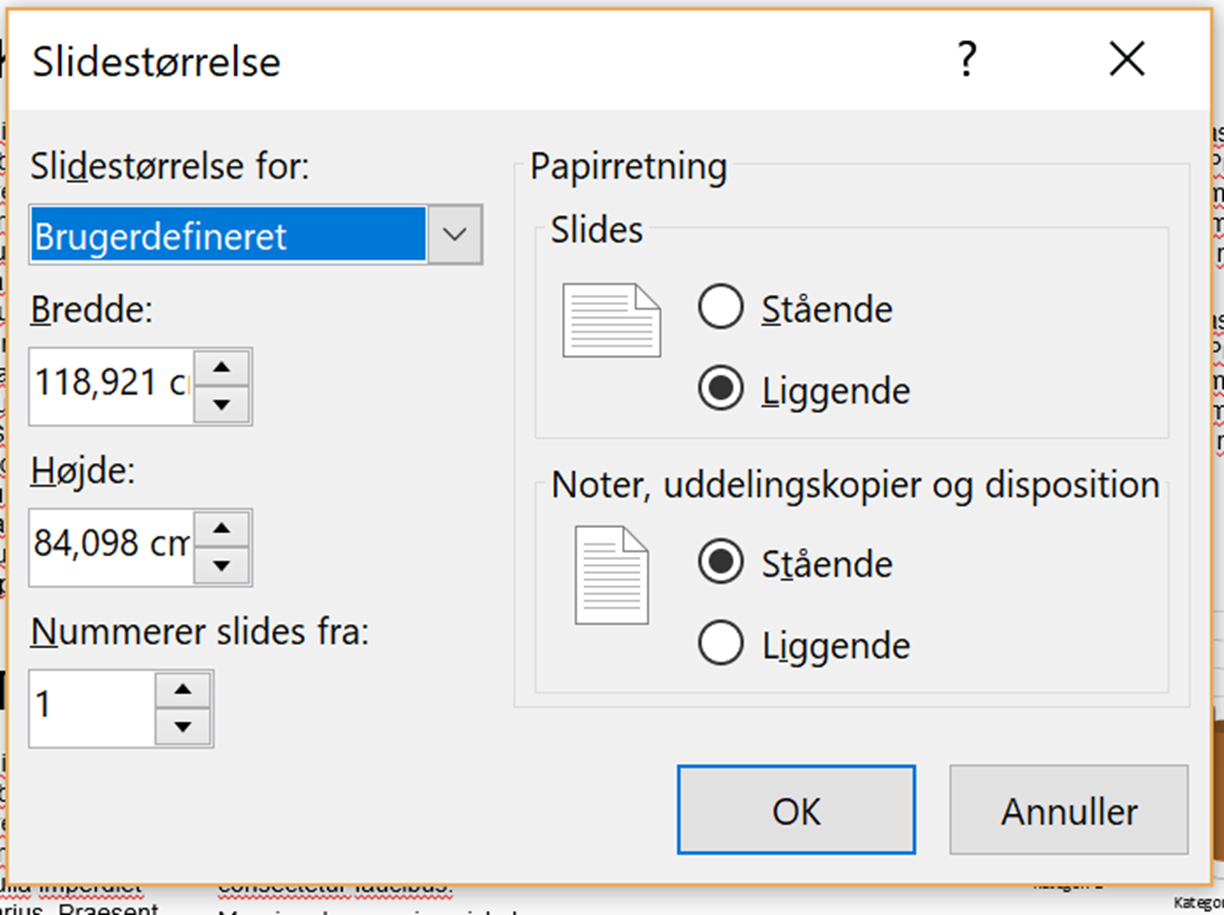
\includegraphics[width=10cm]{images/postersize.png}
%    \caption{Slidestørrelse}\label{fig:poster}
%  \end{center}
%\end{figure}

%Der står fx en A0 printer i printerrummet ved siden af personalefrokostrummet. Se vejledningen i rummet. Posteren præsenteres på et projektseminar. Posteren opdateres og afleveres efter projektseminaret. Vi anbefaler, at I udskriver den opdaterede poster og hænger den op ved jeres projektarbejdsplads.

\section*{Aktiviteter i fasen}

\input{tables/project_phase2_analyse.tex}

\section*{Materialer}

Materialer der er særligt vigtige i problemanalysefasen\footnote{Materialerne ligger på itslearning under planerne \say{General Course/Semester Information}, \say{Semesterprojekt og Projektbeskrivelse} og \say{Projektafleveringfasen og Evaluationfasen}.}:
\begin{itemize}
  \item Semesterplan
  \item Projektbeskrivelse
  \item World of Zuul
    \begin{itemize}
    \item Zuul-framework [Se Planen \say{02 Problemanalysefasen}]
    \item Ide til udforskning af World of Zuul \hyperref[sec:ide]{(Link)}
    \end{itemize}
  \item Projektgrundlag \hyperref[sec:p]{(poster)}
\end{itemize}

\newpage

\section*{Appendix 1: Udforskning af den Udleverede Kildekode i Problemanalysen}
\label{sec:ide}

I projektstarten udforskes den udleverede kildekode som en del af problemanalysen. Vi foreslår, at I som minimum gennemfører følgende opgaver: 

\begin{enumerate}
%    \item \textbf{Execute!}\\
%    Lav en ny klasse, kaldet ”Start”, hvori i inkluderer en main()-metode. Inde i main()-metoden skal i oprette en reference til ”Game”, lave en instans af klassen og køre metoden play() på Game-objektet I har lavet.
%    \\ Forsøg at køre programmet. Hvad sker der?
    
  \item \textbf{”Use the Source, Luke!”}\\
    At kunne læse kildekode er en essentiel del af dét at kunne programmere. I første omgang skal I gennemlæse kildekoden. Dette gør I ved at åbne de forskellige klasser, og forsøge at forstå hvad de gør. Det er sandsynligt, at I ikke forstår hele kildekoden fra starten af, men efterhånden som semesteret skrider frem, bør det blive klart for jer.
    \\
    Brug kommentarer til at beskrive funktionaliteten på de enkelte linjer, og for de enkelte metoder.
    
  \item \textbf{Cause and Effect}\\
    Lav små ændringer i den eksisterende kode. Forslag til ændringer I kan foretage er:
    \begin{itemize}
      \item Ændre navnet på et rum.
      \item Ændre udgangene. Tag fx et rum, som aktuelt ligger vest for et andet, og flyt det så det kommer til at ligge nord for det.
      \item Tilføj et rum \ldots\ og måske flere!
    \end{itemize}
    Sørg for, at I får afviklet spillet mellem hver ændring, så I er sikre på, at spillet stadig virker.
\end{enumerate}

Ovenstående øvelser er med til at gøre jer fortrolige med kildekoden. 

\AtEndDocument{
  \section*{Appendix 2: Præsentation - Projektgrundlag - poster}
  \label{sec:p}
  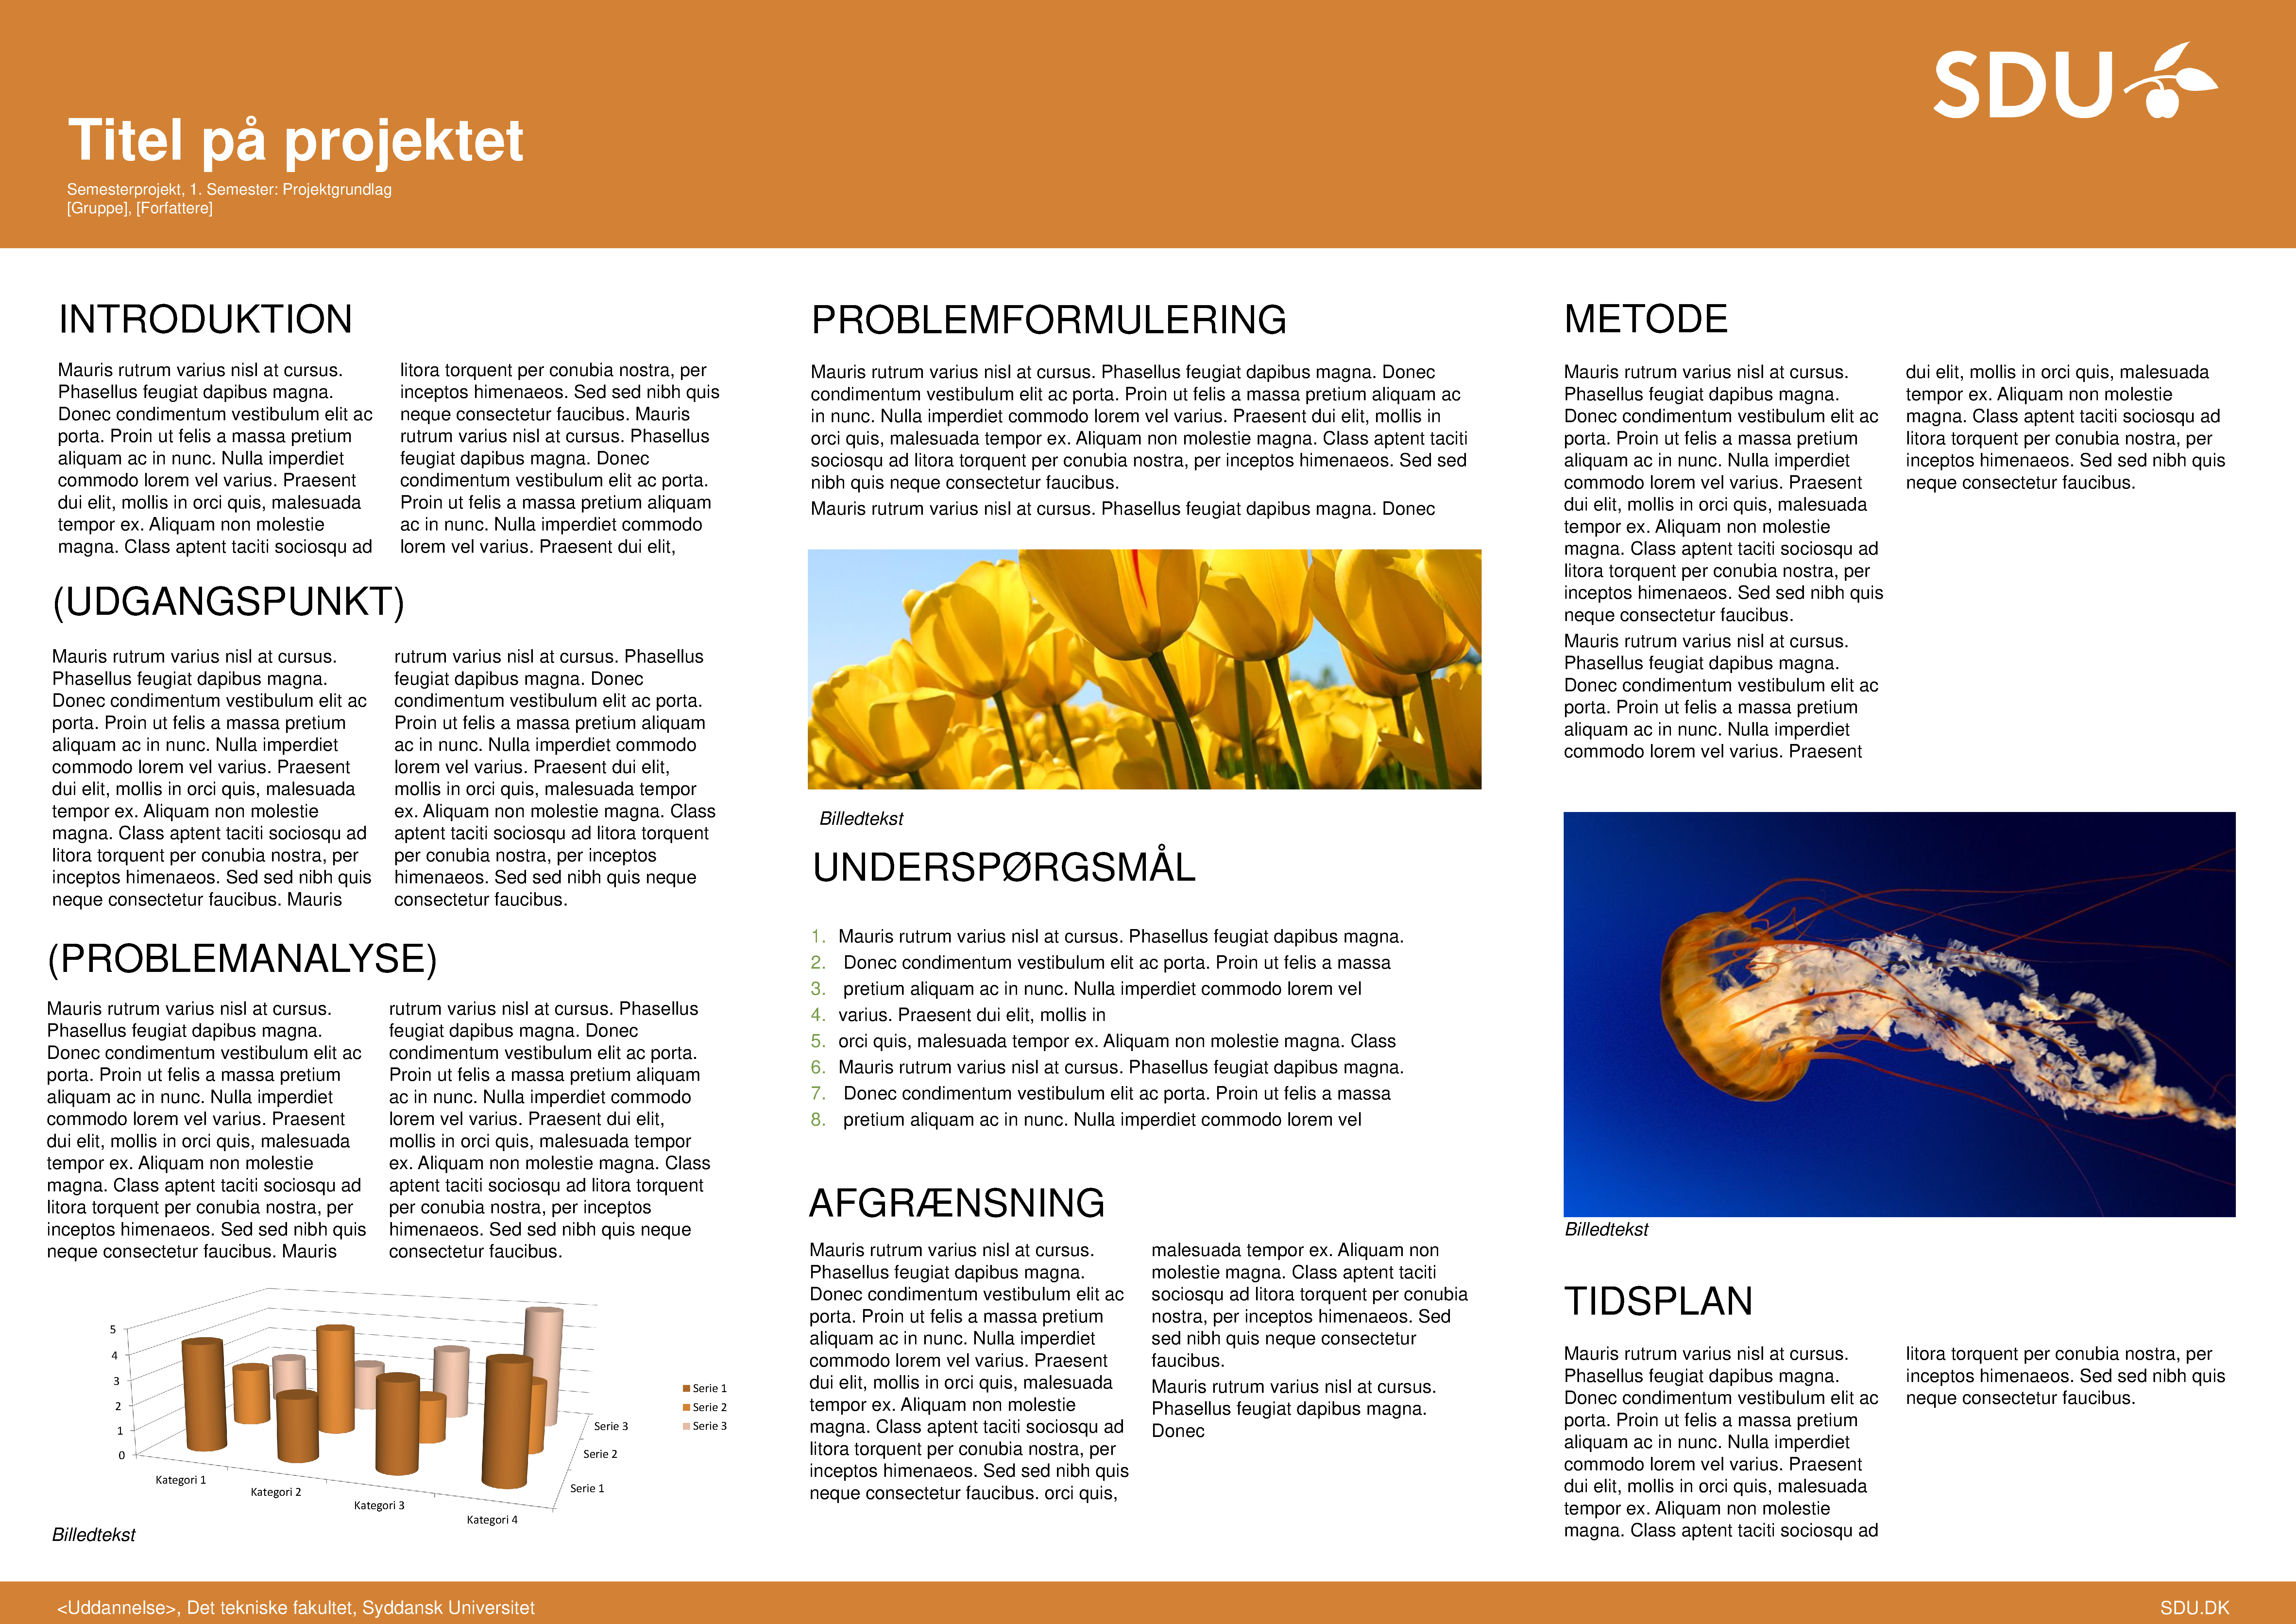
\includepdf[pages=-,pagecommand={}]{pdfs/projektposter.pdf}
}

\end{document}


\section*{Materialer}

Materialer der er særligt vigtige i problemanalysefasen\footnote{Materialerne ligger på itslearning under planerne \say{General Course/Semester Information}, \say{Semesterprojekt og Projektbeskrivelse} og \say{Projektafleveringfasen og Evaluationfasen}.}:
\begin{itemize}
  \item Semesterplan
  \item Projektbeskrivelse
  \item World of Zuul
    \begin{itemize}
    \item Zuul-framework [Se Planen \say{02 Problemanalysefasen}]
    \item Ide til udforskning af World of Zuul \hyperref[sec:ide]{(Link)}
    \end{itemize}
  \item Projektgrundlag \hyperref[sec:p]{(poster)}
\end{itemize}

\newpage

\section*{Appendix 1: Udforskning af den Udleverede Kildekode i Problemanalysen}
\label{sec:ide}

I projektstarten udforskes den udleverede kildekode som en del af problemanalysen. Vi foreslår, at I som minimum gennemfører følgende opgaver: 

\begin{enumerate}
%    \item \textbf{Execute!}\\
%    Lav en ny klasse, kaldet ”Start”, hvori i inkluderer en main()-metode. Inde i main()-metoden skal i oprette en reference til ”Game”, lave en instans af klassen og køre metoden play() på Game-objektet I har lavet.
%    \\ Forsøg at køre programmet. Hvad sker der?
    
  \item \textbf{”Use the Source, Luke!”}\\
    At kunne læse kildekode er en essentiel del af dét at kunne programmere. I første omgang skal I gennemlæse kildekoden. Dette gør I ved at åbne de forskellige klasser, og forsøge at forstå hvad de gør. Det er sandsynligt, at I ikke forstår hele kildekoden fra starten af, men efterhånden som semesteret skrider frem, bør det blive klart for jer.
    \\
    Brug kommentarer til at beskrive funktionaliteten på de enkelte linjer, og for de enkelte metoder.
    
  \item \textbf{Cause and Effect}\\
    Lav små ændringer i den eksisterende kode. Forslag til ændringer I kan foretage er:
    \begin{itemize}
      \item Ændre navnet på et rum.
      \item Ændre udgangene. Tag fx et rum, som aktuelt ligger vest for et andet, og flyt det så det kommer til at ligge nord for det.
      \item Tilføj et rum \ldots\ og måske flere!
    \end{itemize}
    Sørg for, at I får afviklet spillet mellem hver ændring, så I er sikre på, at spillet stadig virker.
\end{enumerate}

Ovenstående øvelser er med til at gøre jer fortrolige med kildekoden. 

\AtEndDocument{
  \section*{Appendix 2: Præsentation - Projektgrundlag - poster}
  \label{sec:p}
  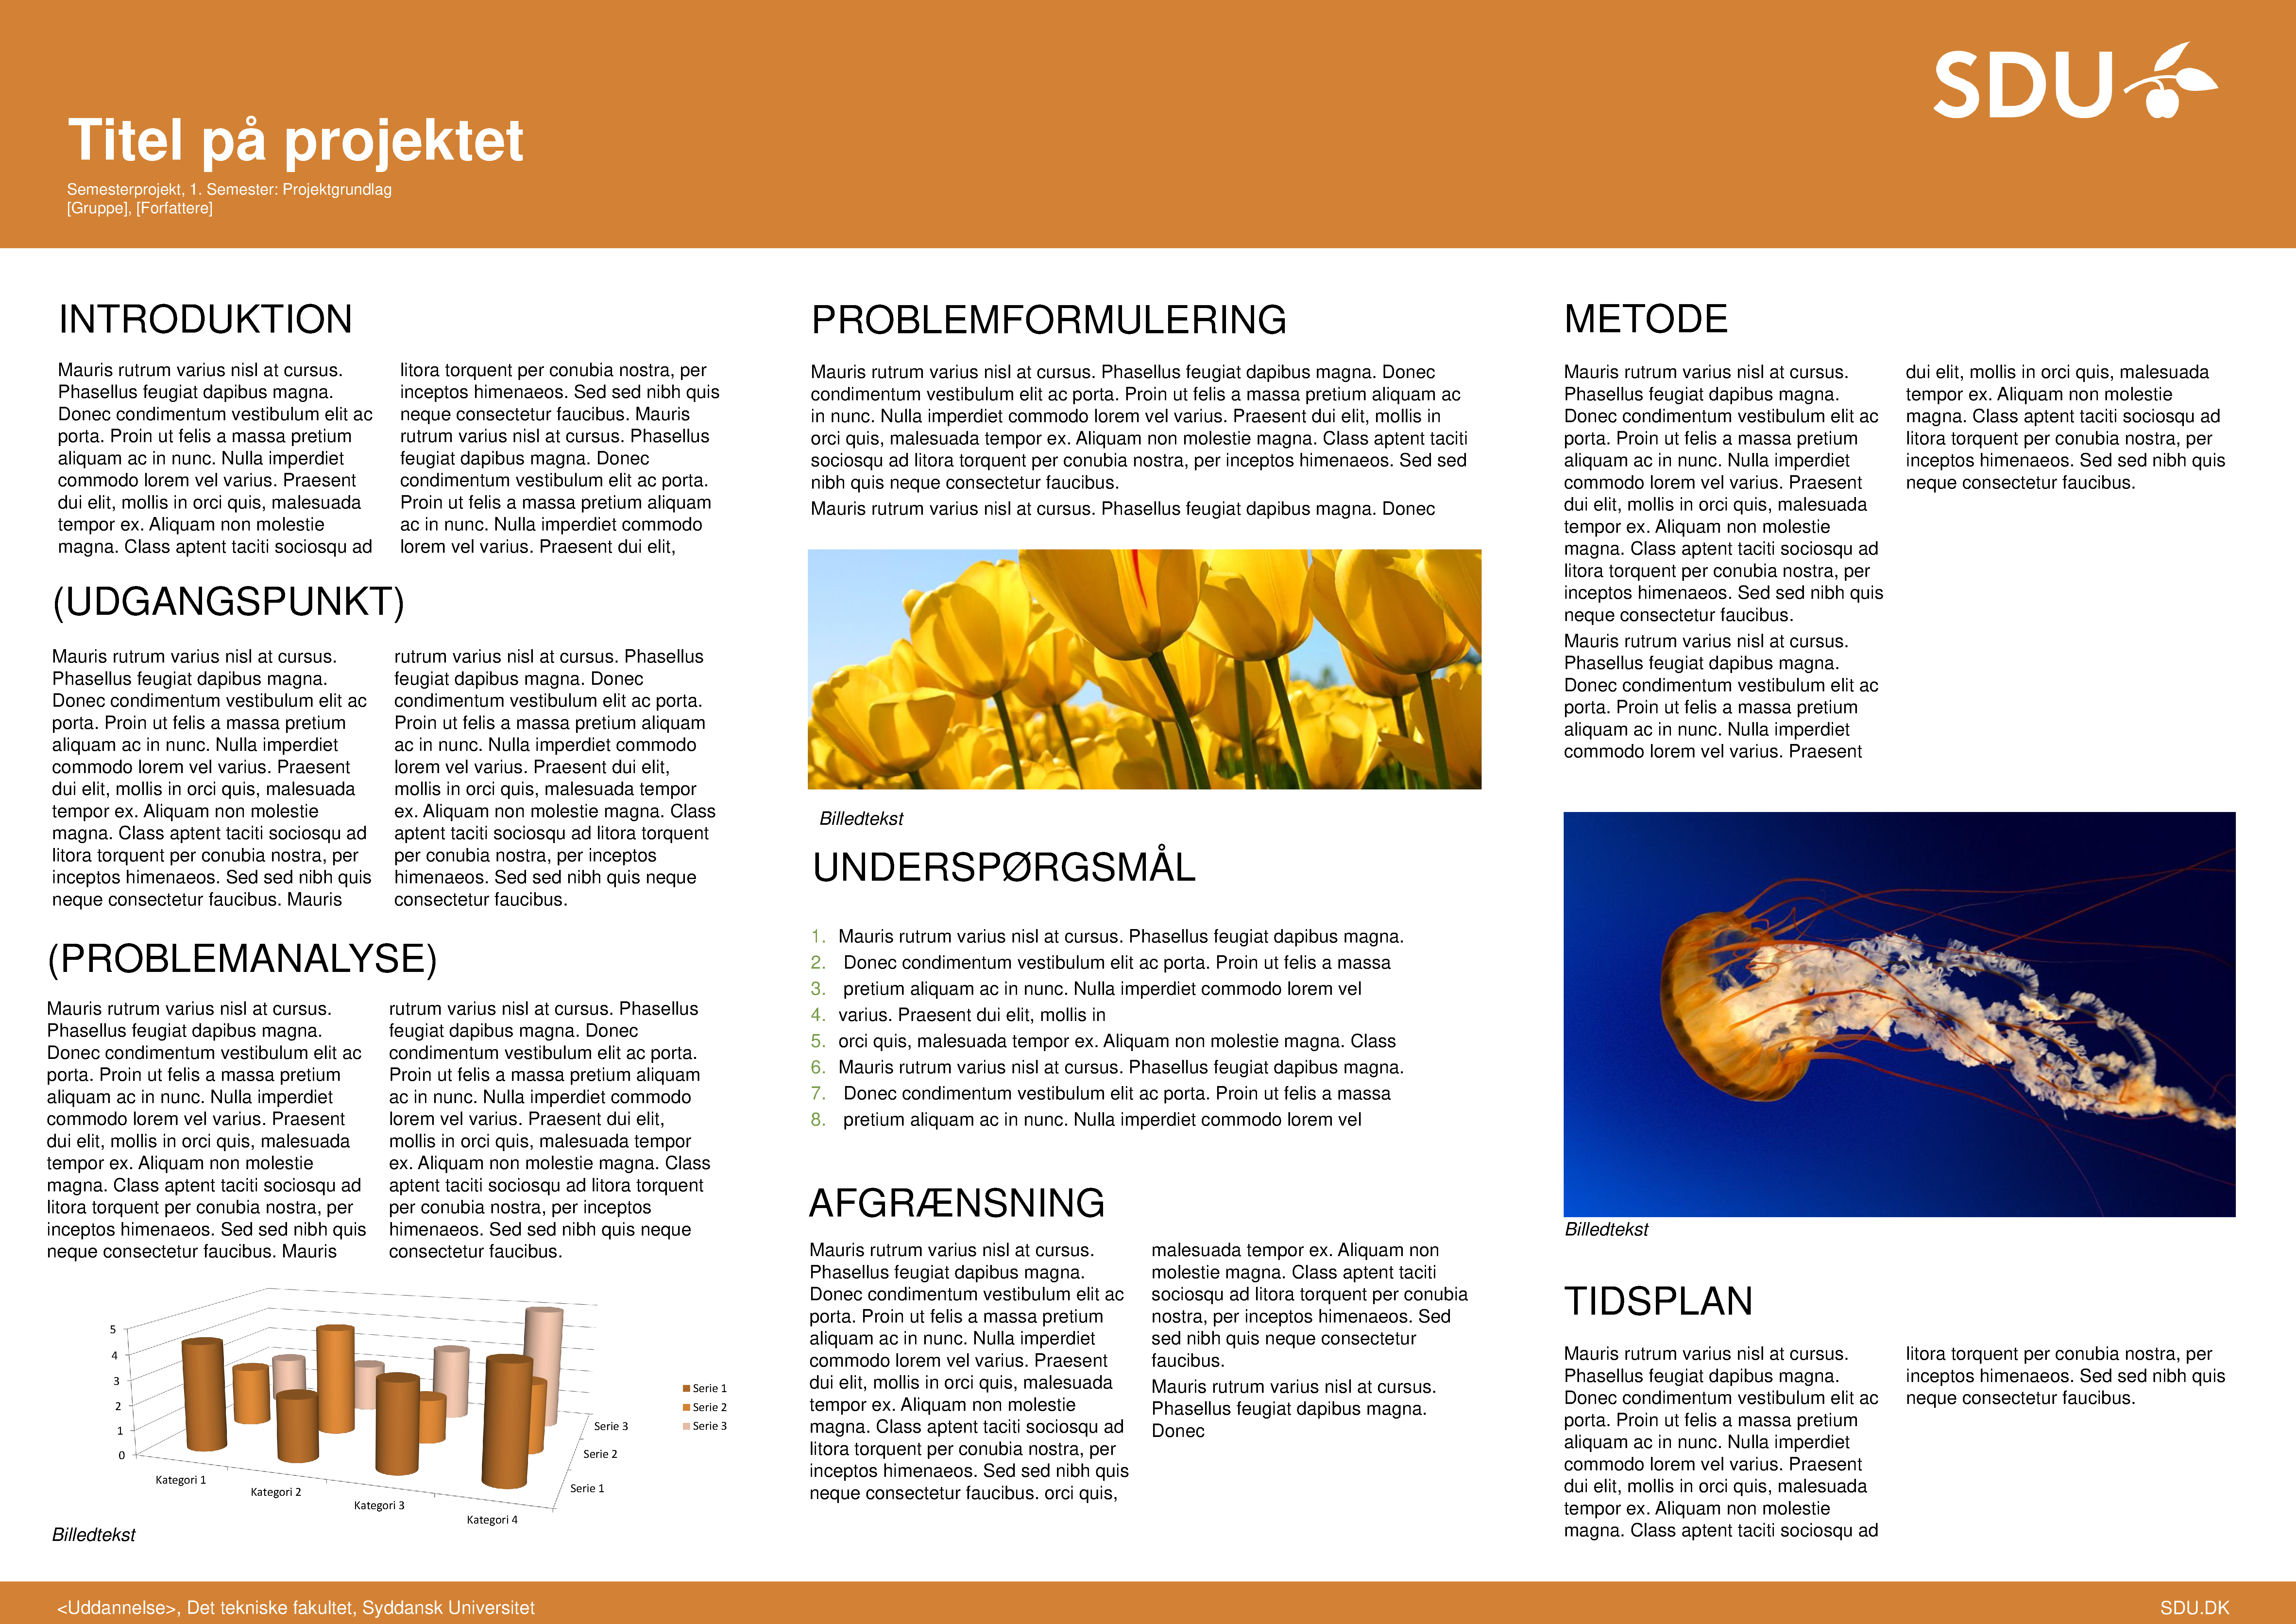
\includepdf[pages=-,pagecommand={}]{pdfs/projektposter.pdf}
}

\end{document}


\section*{Materialer}

Materialer der er særligt vigtige i problemanalysefasen\footnote{Materialerne ligger på itslearning under planerne \say{General Course/Semester Information}, \say{Semesterprojekt og Projektbeskrivelse} og \say{Projektafleveringfasen og Evaluationfasen}.}:
\begin{itemize}
  \item Semesterplan
  \item Projektbeskrivelse
  \item World of Zuul
    \begin{itemize}
    \item Zuul-framework [Se Planen \say{02 Problemanalysefasen}]
    \item Ide til udforskning af World of Zuul \hyperref[sec:ide]{(Link)}
    \end{itemize}
  \item Projektgrundlag \hyperref[sec:p]{(poster)}
\end{itemize}

\newpage

\section*{Appendix 1: Udforskning af den Udleverede Kildekode i Problemanalysen}
\label{sec:ide}

I projektstarten udforskes den udleverede kildekode som en del af problemanalysen. Vi foreslår, at I som minimum gennemfører følgende opgaver: 

\begin{enumerate}
%    \item \textbf{Execute!}\\
%    Lav en ny klasse, kaldet ”Start”, hvori i inkluderer en main()-metode. Inde i main()-metoden skal i oprette en reference til ”Game”, lave en instans af klassen og køre metoden play() på Game-objektet I har lavet.
%    \\ Forsøg at køre programmet. Hvad sker der?
    
  \item \textbf{”Use the Source, Luke!”}\\
    At kunne læse kildekode er en essentiel del af dét at kunne programmere. I første omgang skal I gennemlæse kildekoden. Dette gør I ved at åbne de forskellige klasser, og forsøge at forstå hvad de gør. Det er sandsynligt, at I ikke forstår hele kildekoden fra starten af, men efterhånden som semesteret skrider frem, bør det blive klart for jer.
    \\
    Brug kommentarer til at beskrive funktionaliteten på de enkelte linjer, og for de enkelte metoder.
    
  \item \textbf{Cause and Effect}\\
    Lav små ændringer i den eksisterende kode. Forslag til ændringer I kan foretage er:
    \begin{itemize}
      \item Ændre navnet på et rum.
      \item Ændre udgangene. Tag fx et rum, som aktuelt ligger vest for et andet, og flyt det så det kommer til at ligge nord for det.
      \item Tilføj et rum \ldots\ og måske flere!
    \end{itemize}
    Sørg for, at I får afviklet spillet mellem hver ændring, så I er sikre på, at spillet stadig virker.
\end{enumerate}

Ovenstående øvelser er med til at gøre jer fortrolige med kildekoden. 

\AtEndDocument{
  \section*{Appendix 2: Præsentation - Projektgrundlag - poster}
  \label{sec:p}
  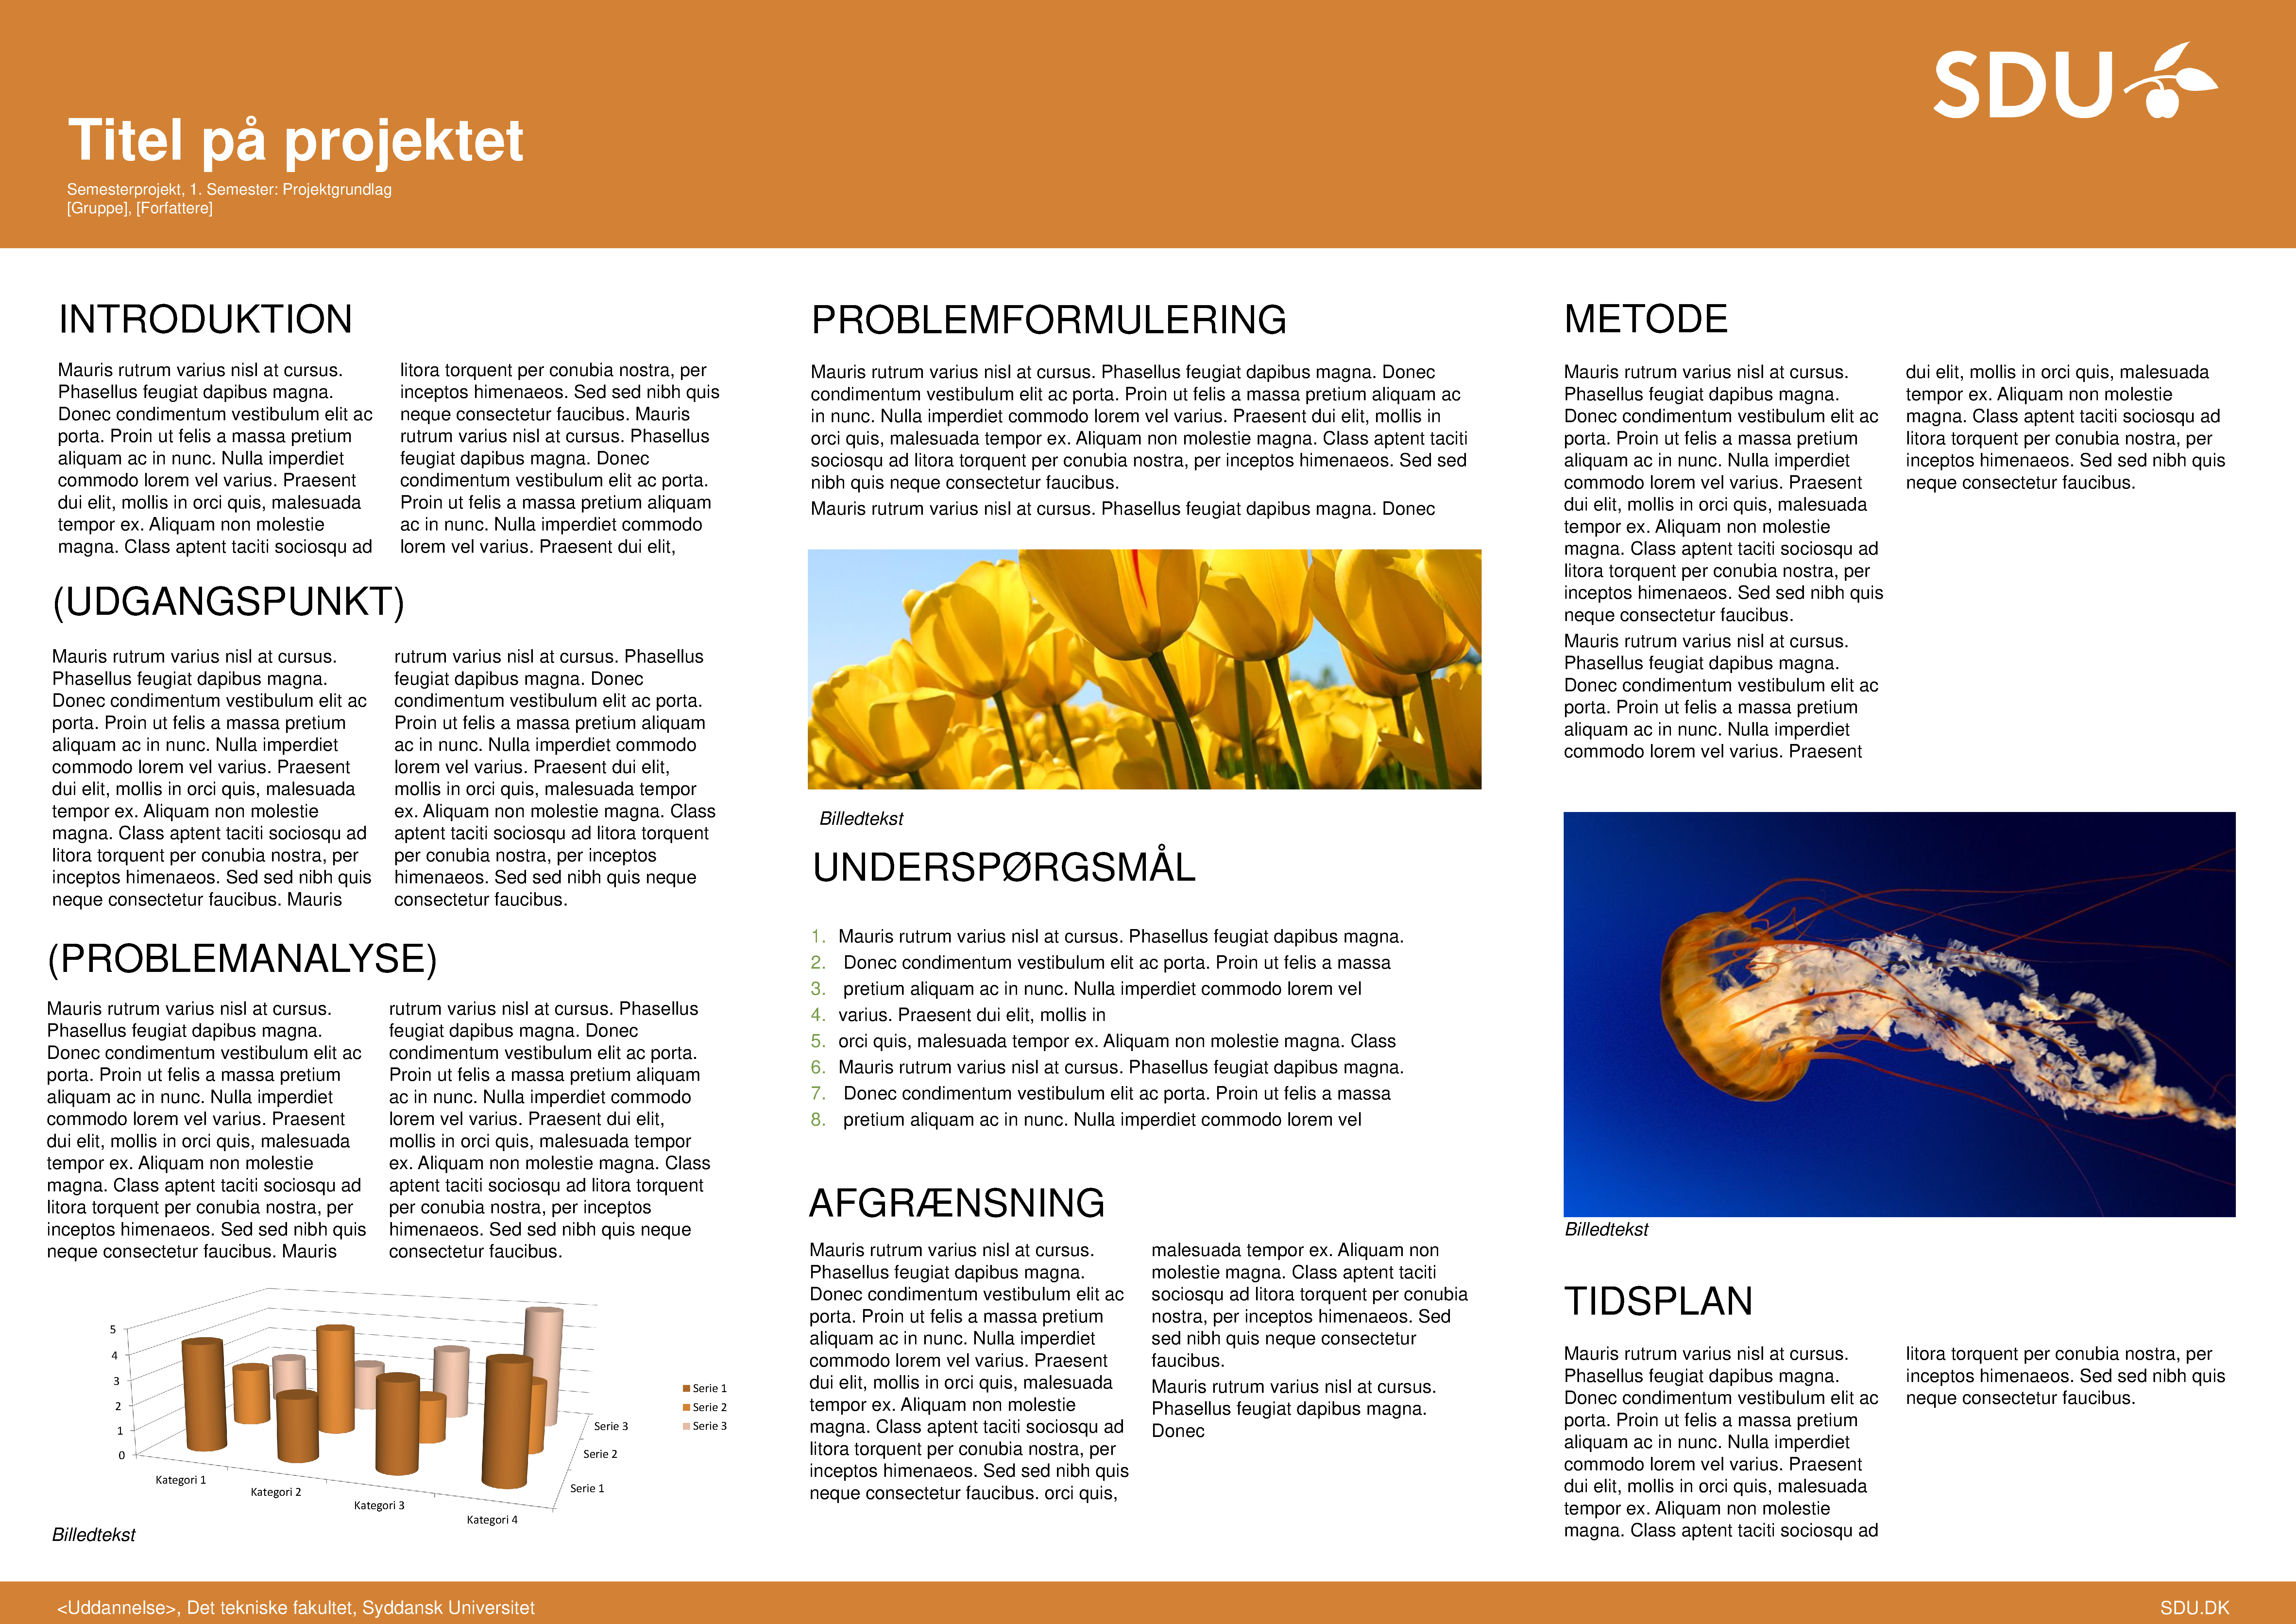
\includepdf[pages=-,pagecommand={}]{pdfs/projektposter.pdf}
}

\end{document}


\section*{Materialer}

Materialer der er særligt vigtige i problemanalysefasen\footnote{Materialerne ligger på itslearning under \textsl{"General Course/Semester Information"}, \textsl{"Semesterprojekt og Projektbeskrivelse"} og \textsl{"Projektafleveringfasen og Evaluationfasen"}.}:
\begin{itemize}
  \item Semesterplan
  \item Projektbeskrivelse
  \item World of Zuul
    \begin{itemize}
    \item Zuul-framework [See Plans (02 Problemanalysefasen]
    \item Ide til udforskning af World of Zuul \hyperref[sec:ide]{(Link)}
    \end{itemize}
  \item Projektgrundlag \hyperref[sec:p]{(poster)}
\end{itemize}

\newpage

\section*{Appendix 1: Udforskning af den udleverede kildekode i problemanalysen}\label{sec:ide}
I projektstarten udforskes den udleverede kildekode som en del af problemanalysen. Vi foreslår at I som minimum gennemfører følgende opgaver: 


\begin{enumerate}
    \item \textbf{Execute!}\\
    Lav en ny klasse, kaldet ”Start”, hvori i inkluderer en main()-metode. Inde i main()-metoden skal i oprette en reference til ”Game”, lave en instans af klassen og køre metoden play() på Game-objektet I har lavet.
    \\ Forsøg at køre programmet. Hvad sker?
    
     \item \textbf{”Use the source, Luke!”}\\
    At kunne læse kildekode er en essentiel del af det at kunne programmere. I første omgang skal I gennemlæse kildekoden, ved at åbne de forskellige klasser, og forsøge at forstå hvad de gør. Det er muligt, at I ikke forstår hele kildekoden fra starten af, men efterhånden som semesteret skrider frem, bør det blive klart for jer. 
\\
\\
   Brug kommentarer til at beskrive funktionaliteten på de enkelte linjer – og for de enkelte metoder.

    
     \item \textbf{Cause and effect}\\
    Lav småændringer i den eksisterende kode. Forslag til ændringer I kan foretage er:
    \begin{itemize}
    \item Ændre navnet på et rum
    \item Ændre udgangene – tag f.eks. et rum, som nu ligger til vest for et andet, og flyt det til nord.
    \item Tilføj et rum… og måske flere!
    \end{itemize}
    \\ Sørg for, at I får afviklet spillet mellem hver ændring, så I er sikre på, at spillet stadig virker.
    
    \\ Ovenstående øvelser er med til at gøre jer fortrolige med kildekoden. 

\end{enumerate}
\AtEndDocument{
\section*{Appendix 2: Præsentation - Projektgrundlag - poster}\label{sec:p}
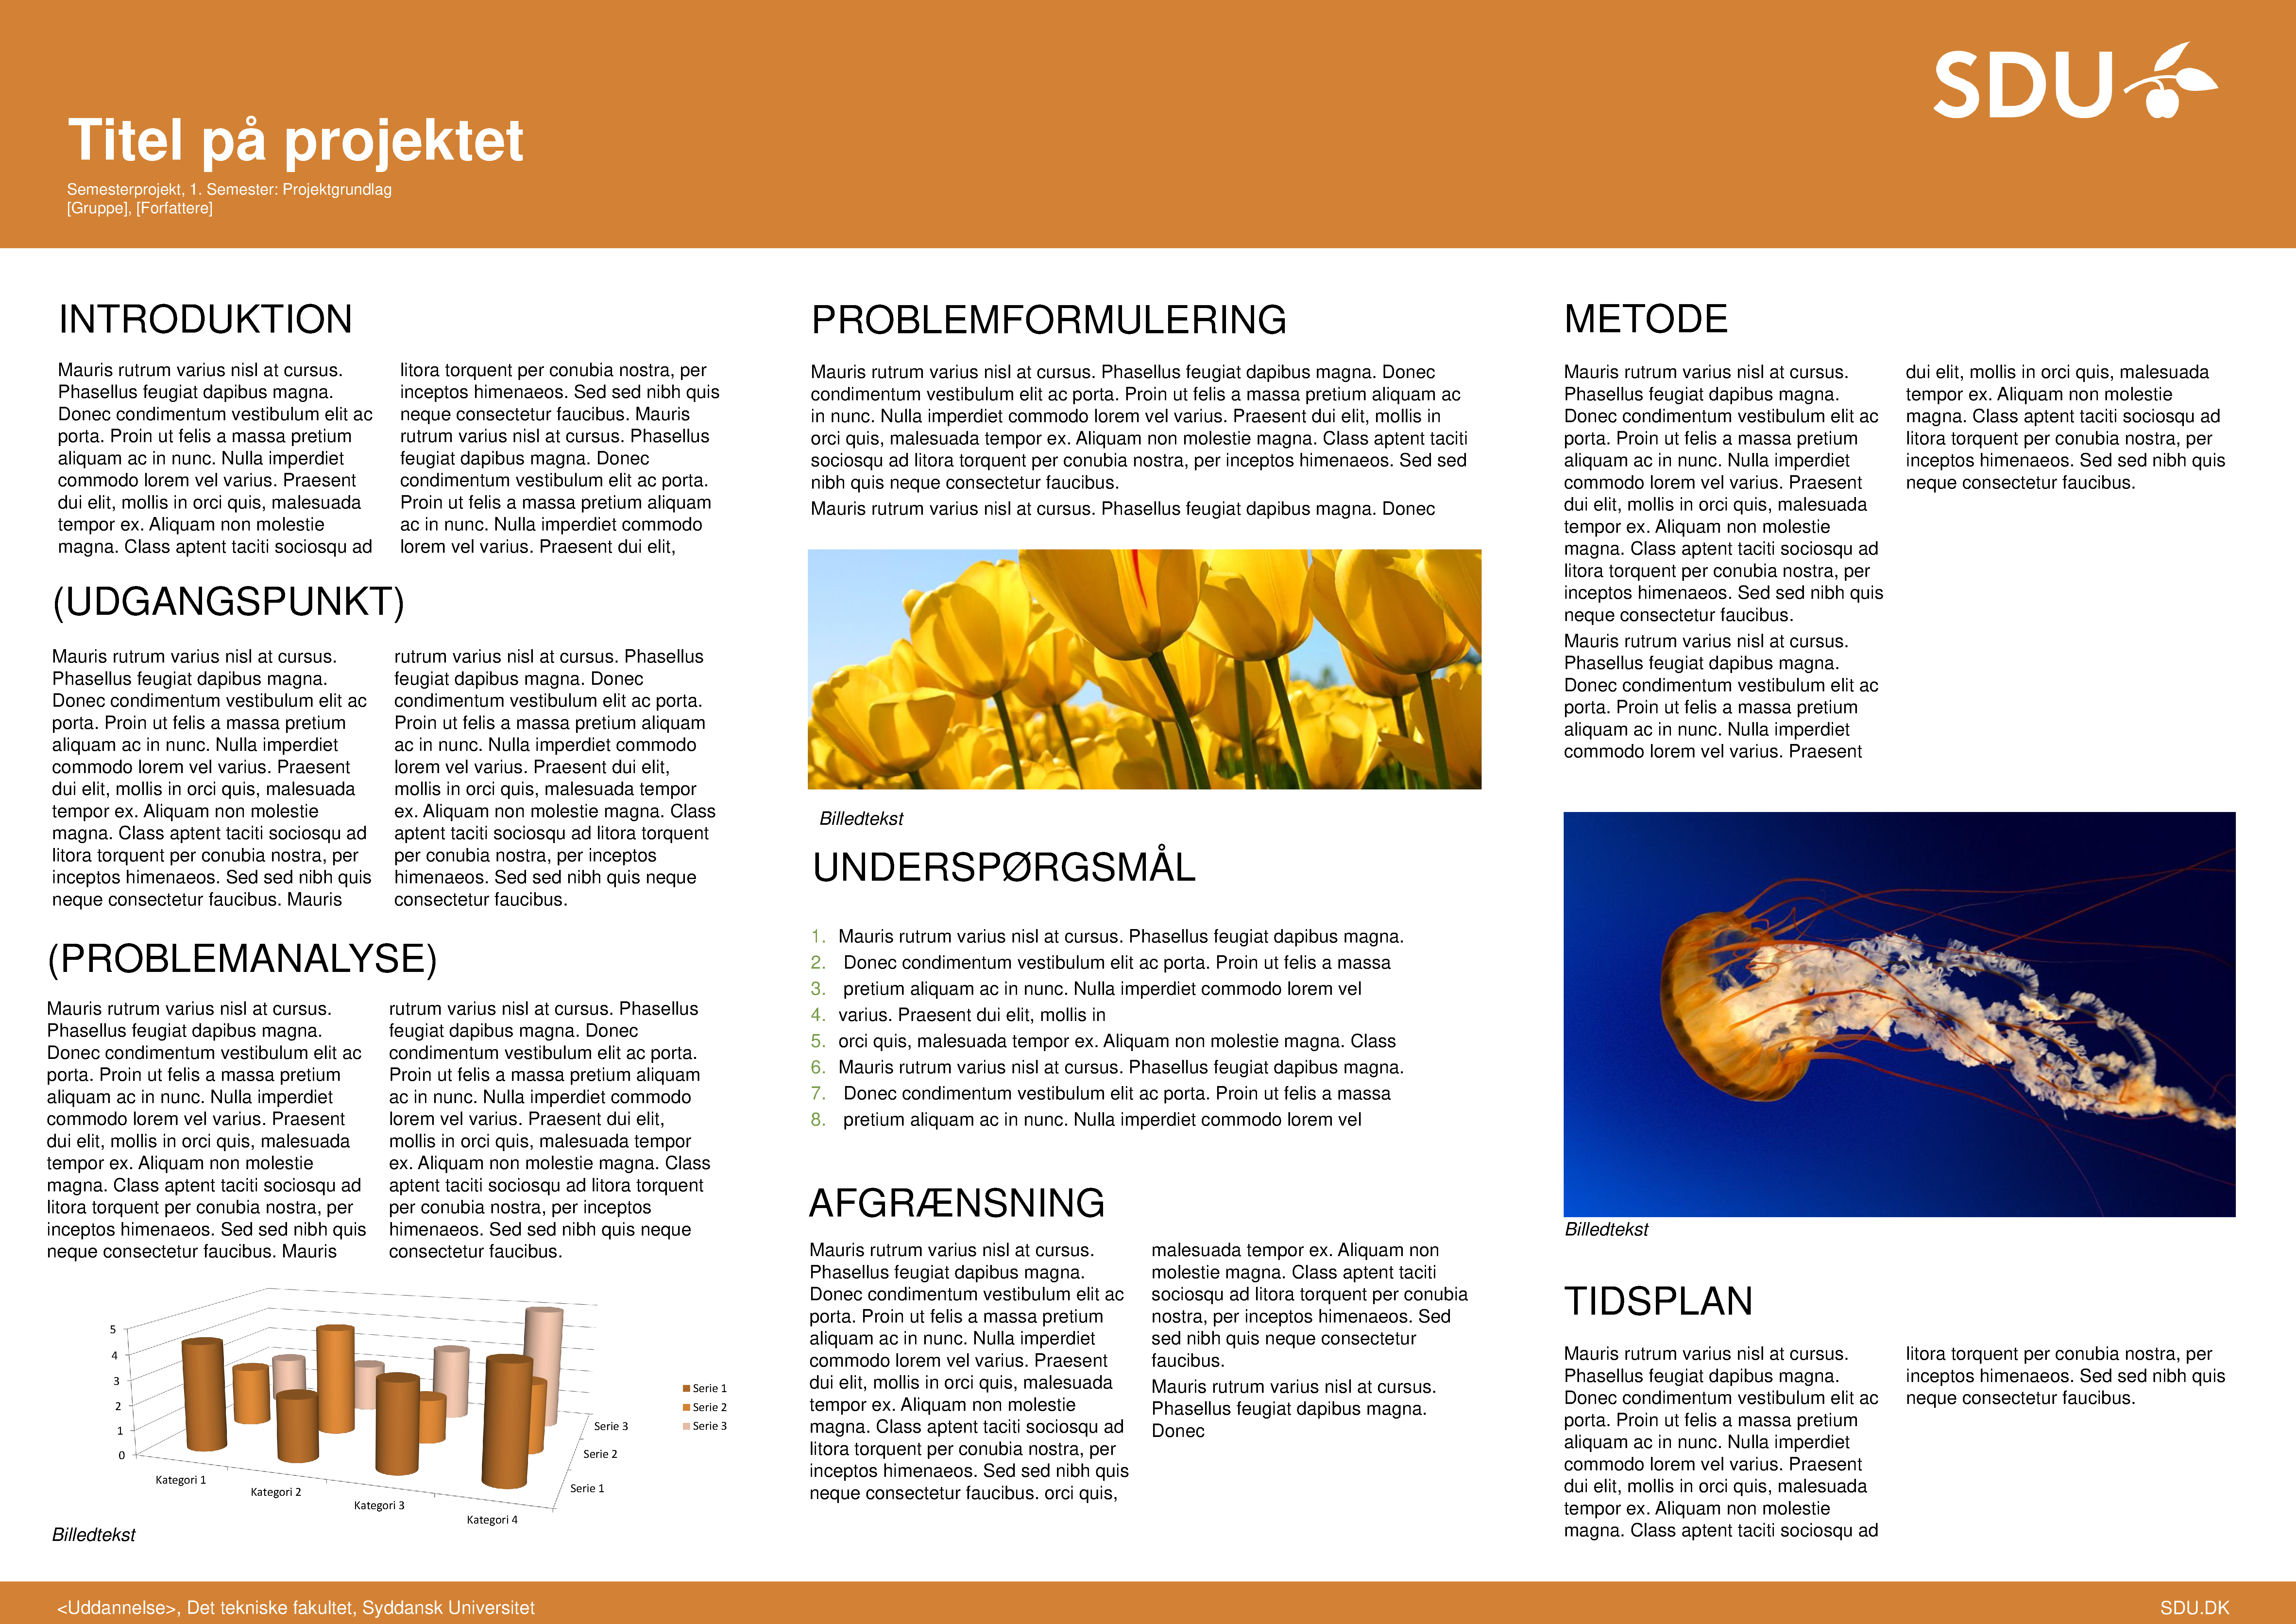
\includepdf[pages=-,pagecommand={}]{pdfs/projektposter.pdf}
}

\end{document}
